\documentclass[spanish,english,12pt,letterpaper,oneside]{book}
\usepackage{layout}
\usepackage[spanish]{babel}
\usepackage{calc}
\usepackage[latin1]{inputenc}
\usepackage{graphicx}
\usepackage{subcaption}
\usepackage{latexsym}
\usepackage{amssymb}
\usepackage{fancybox}
\usepackage{fancyvrb}
\usepackage{fancyhdr}
\usepackage{relsize}
\usepackage{pgf,pgfarrows,pgfnodes}
\usepackage{pgfplots}
\usepackage{tikz}
\usepackage{pbox}
\usepackage{rotating}
\usepackage{tabularx}
\usepackage{color}
\usepackage{float}
\usepackage{index}
%\usepackage{wasysym}
\usepackage{indentfirst} %always indent first paragraph after chapter or section
\usepackage{amsmath}
\usepackage{multirow}
\usepackage{notoccite} %avoid citation on list of figures and tables affect order
\usepackage{listings}
\usepackage[pdftex,hyperindex,breaklinks]{hyperref}%,colorlinks,urlcolor=blue,linkcolor=blue]{hyperref}
\usepackage[justification=centering]{caption}
\usepackage[left=4cm,top=3.0cm,right=3.4cm,bottom=3.9cm]{geometry}

%Para activar el doble espacio
%\renewcommand{\baselinestretch}{2} 

\usepackage[ruled]{algorithm}

%\usepackage[noend]{algpseudocode}
\usepackage{algpseudocode}

\usepackage{tcolorbox} 

% new tcolorbox environment
% #1: tcolorbox options
% #2: color
% #3: box title
\newtcolorbox{mybox}[3][]
{
  colframe = #2!25,
  colback  = #2!10,
  coltitle = #2!20!black,  
  title    = #3,
  #1,
}


\renewcommand{\headrulewidth}{1pt}
%\renewcommand{\footrulewidth}{0.5pt}


\newcounter{myfootertablecounter}

\newcommand\myfootnotemark{%
  %\refstepcounter{footnote}%
  \addtocounter{footnote}{1}%
  \footnotemark[\thefootnote]%
}%

\newcommand\myfootnotetext[1]{%
  \addtocounter{myfootertablecounter}{1}
  \footnotetext[\value{myfootertablecounter}]{#1}
}

% from now on, myfootnote has to be used rather than footnote to
% adapt the myfootercounter
\newcommand\myfootnote[1]{%
  \addtocounter{myfootertablecounter}{1}
  \footnote{#1}
}%


\pagestyle{fancy}

\rhead[]{\leftmark}
\lhead[\rightmark]{}
%\lfoot[\thepage]{ATLAS Grid Information System}
\rfoot[ATLAS Grid Information System]{\thepage}
\cfoot{} 


%\renewcommand{\listalgorithmname}{\'Indice de algoritmos}
\renewcommand{\chaptermark}[1]{\markleft{\thechapter #1}}
\renewcommand{\sectionmark}[1]{\markright{\thesection #1}}
\renewcommand{\chaptermark}[1]{\markboth{\chaptername \ \thechapter. #1}{}}

\newcommand{\contrib}[3]{#1\quad$<$\texttt{#2}$>$%
{\small\\\quad\textit{#3}}\\[1ex]}

\pgfdeclareimage[width=5cm]{logo-utfsm}{images/logo-grande}

\title{3D Scene Reconstruction}

\author{
  Juan Reyes \\ \texttt{jareyes@alumnos.inf.utfsm.cl}
}

\date{$\infty$}

\frenchspacing

\makeindex

\begin{document}
    \newenvironment{dedication}
        {\vspace{6ex}\begin{quotation}\begin{center}\begin{em}}
        {\par\end{em}\end{center}\end{quotation}}

\frontmatter

\thispagestyle{empty}

\begin{center}

{\large\bfseries Universidad T�cnica Federico Santa Mar�a}\\[2mm]
{\large\bfseries Departamento de Inform�tica}\\[2mm]
\pgfuseimage{logo-utfsm}
\end{center}

\vspace*{\stretch{3}}

\begin{center}
{\LARGE\bfseries 3D Scene Reconstruction }\\[2mm]
%{\LARGE\bfseries Using a Kinect sensor}
\end{center}

\vspace*{\stretch{5}}

\begin{center}
{\large por}\\[2mm]
{\huge Juan Alfonso Reyes L�pez}
\end{center}


\vspace*{\stretch{5}}

\begin{center}
{\large Tesis para optar al  grado de}\\[2mm]
\vspace*{10mm}
{\LARGE Mag�ster en Ciencias de la Ingenier�a Inform�tica}\\[2mm]
%{\large for the degree of}\\
%{\Large Master in Science of Informatic Engineering}
\end{center}

\vspace*{\stretch{5}}


\begin{center}
{\large Valpara\'{i}so - Chile}\\
{\large Marzo de 2015}\\[2mm]
\end{center}

\vspace*{\stretch{1}}

\pagebreak

\thispagestyle{empty}

\begin{center}
{\Large Universidad T\'{e}cnica Federico Santa Mar\'{\i}a} \\
{\Large Departamento de Inform�tica}\\
{\Large Valpara\'{\i}so - Chile}\\
\end{center}

\vspace*{\stretch{1}}

\begin{center}
{\large TITULO DE LA TESIS:}\\
{\large \textbf{3D Scene Reconstruction}}
\end{center}

\vspace*{\stretch{1}}

\begin{center}
{\large AUTOR:}\\
{\large \textbf{Juan Alfonso Reyes L�pez}}\\
\end{center}

\vspace*{\stretch{2}}

{\large TRABAJO DE GRADO, presentado en cumplimiento parcial de los
requisitos para el Grado de
Mag�ster en Ciencias de la  Ingenier�a Inform�tica de la Universidad T�cnica Federico
Santa Mar�a.}

\vspace*{\stretch{5}}

\begin{table}[ptbh]
\begin{tabular}[c]{lc}
{\large Prof. Dr. Luis Salinas} & \begin{picture}(200,5) \line(1,0){200} \end{picture}\\
& {\large Profesor Gu�a } \\
& \\
& \\
& \\
{\large Prof. Dr. Claudio Torres } & \begin{picture}(200,5) \line(1,0){200} \end{picture} \\ 
& {\large Correferente } \\
& \\
& \\
& \\
{\large Dr.} & \begin{picture}(200,5) \line(1,0){200} \end{picture}\\
& {\large Correferente Externo }
\end{tabular}
\end{table}

\vspace*{\stretch{1}}

\begin{center}
{\large Marzo de 2015}
\end{center}
 
\pagebreak


\endinput


\begin{dedication}
A mi madre por inculcarme la importancia de la educaci\'on,

A mi padre por demostrarme el valor de la creatividad,

A mi hermana por su apoyo incondicional,

A Carolina por compartir su vida conmigo.
\end{dedication}



\chapter*{Abstract}

3D point cloud registration is an important step in every 3D reconstruction system. This thesis proposes to register 
3D point clouds, applying a filtering step where only edges that appear 
in the two point clouds to be aligned pass the filter. For this purpose a combination of visual and geometrical information is 
used along with the Iterative Closest Point (ICP)
  algorithm and a pose graph optimization method. The proposed technique reduces the amount of calculations 
involved because only between 10\% and 20\% of original points are used as input for the ICP algorithm, increasing 
the quality of the alignment, working with the most representative subset of the data. At difference to other techniques 
involving edge filtering along with ICP, this proposal increments the odds of a correct alignment filtering out non common 
data from the pair of point clouds to be aligned. Quantitative results shows the advantages of the proposed method. A 
public available dataset was used, 
providing the source 
code and all the necessary information to compare and replicate the presented results.

\section*{Keywords}

3D reconstruction, simultaneous location and mapping, iterative closest point, Kinect, point cloud



\chapter*{Resumen}

En general un sistema de reconstrucci\'on 3D tiene tres pasos principales: adquisici\'on de datos, registro y reconstrucci\'on. Durante el paso de registro los puntos 3D son registrados en un sistema de coordenadas com\'un. El algoritmo de b\'usqueda iterativa de puntos cercanos (ICP) es 
ampliamente usado para realizar el registro de los puntos, sin embargo es computacionalmente costoso y propenso a converger a un m\'inimo local. Esta tesis propone enfrentar estos problemas, aplicando un paso de filtrado donde solo los bordes que aparecen en las dos nubes de puntos 
que est\'an siendo alineadas pasan el filtro. Una combinaci\'on de informaci\'on visual y geom\'etrica es 
usada junto con ICP y un m\'etodo de optimizaci\'on de grafos. 
La t\'ecnica propuesta 
disminuye la cantidad de c\'omputos necesarios porque s\'olo entre un 10\% y un 20\% de los puntos originales son usados 
como entrada para el algoritmo ICP, 
aumentando la calidad de la alineaci\'on, trabajando con el subconjunto de datos m\'as representativo. A diferencia de otras 
t\'ecnicas que involucran filtrado de bordes junto con ICP, esta propuesta incrementa las probabilidades de una alineaci\'on 
correcta quitando los puntos no comunes entre el par de nubes de puntos a alinear. Los resultados cuantitativos muestran 
las ventajas del m\'etodo propuesto. Un conjunto de datos p\'ublicamente disponible fue utilizado para los experimentos, el c\'odigo 
y toda la informaci\'on necesaria para comparar y replicar los resultados es provista.


\section*{Palabras clave}


Reconstrucci\'on 3D, localizaci\'on y mapeo simult\'aneo, algoritmo de b\'usqueda iterativa de puntos cercanos, Kinect, nube de puntos.


\addcontentsline{toc}{section}{\contentsname}
\tableofcontents

%\addcontentsline{toc}{subsection}{\listalgorithmname}
%\listofalgorithms
\addcontentsline{toc}{subsection}{\listfigurename}
\listoffigures
\addcontentsline{toc}{subsection}{\listtablename}
\listoftables

\mainmatter

\chapter{Introduction}
\label{introduccion}
\index{Introducction}

The 3D scene reconstruction problem consists in take the
necessary information from a real scene in order to reconstruct
it in a three dimensional space, usually to be displayed 
in a computer. 

The objetive is to represent in the most accurate way the geometric scene details, obtaining rich 
information about the scene that is not explicity contained on a single image and then use this 
to reconstruct the scene or use it to perform a more advanced task that depends of the scene geometry. 
Some applications of 3D scene reconstruction are : Autonumous vehicle or robot navigation, where there is crucial to have 
the scene geometry in order to locate paths and obstacles. Augmented Reallity, where a virtual 3D object
 is added to a real video of the scene. Parts inspection in a manufacturing plant, where is necesary to detect
 fabrication defects on some objects. Statues and Buildings preservation, in order to have a digital representation 
of the objects and beign able to reproduce or mantain them.

 
In general the information is acquired
 from the scene with optical devices, such as RGB cameras or depth sensors.
Most of 3D scene reconstruction methods can be classified in passive methods and active methods \cite{lanman}.
The passive methods works without controlling the light in the scene, they just receipt light (ordinary cameras). 
By the other hand active methods alter the light in the scene, with a light emisor and its corresponding 
receptor, projecting patterns of light in order to simplify the matching process prior to the triangulation. 
There are also some active methods that touch the object in order to reconstruct it, but they are beyond 
the scope of this thesis. 

The most accurate and expensive method to perform 3D scene reconstruction is the Laser Scanning, because it has 
an hight accuracy (about xx mm). But nowadays there are emerging cheaper devices that potentially could perform 
a similar reconstruction at a pair of orders of magnitude low cost. 

One of the most classical approaches is to use multiple 2D
 images taken from known camera viewpoints and estimate the distance of each
 relevant pixel with triangulation (Stereo Vision, Multiview Vision), with this 
approaches the depth map must be generated using the geometrical information contained
 on the images. Nowadays is common to find devices that generate depth maps accesible
 to everyday users and automatize the depth map generation step, this devices are called depth sensors. 
Depth sensors give to each pixel of the image a depth value, related
with the distance of the real object from the sensor, offering a more
accurate data to perform 3D reconstruction. With the appearance
of cheap depth sensors for gaming and entertainment (such as
Kinect). There is a growing interest in the develop of low cost
3D reconstruction systems. 


One of the key steps of a 3D reconstruction algorithm is the registration, where the 3D points corresponding to
 the scene are  registered in a common coordinate system, preserving the original scene disposition. Another important 
step is to add colour and continuity to the reconstructed scene, usually using a lot of geometric primitives such as 
triangles, in order to generate a textured 3D model. This thesis is  about the registration step. 



Sean los conjuntos de puntos  ${a_i},{b_i} \in \mathbb{R}^3;i = 1,2,...,N$.
Se desea encontrar $R,\vec{t}$ que minimize:
$$
\sum\limits_{i=1}^N || Ra_i - b_i - \vec{t} ||
$$
Donde $R$ es una matriz de rotacion de $3x3$ y $\vec{t} \in \mathbb{R}^3$.


\section{Thesis Outline}

The rest of the document is structured as follows:

\begin{itemize}
\item Chapter 2: Presents recent and important works in 3D reconstruction. 

\item Chapter 3: Explains the sensor used to capture the data and how it works.

\item Chapter 4: Describes all the used techniques and the proposed method.

\item Chapter 5: Presents the dataset, tools and results obtained with the proposed method.

\item Chapter 6: Presents the conclusions and the future works.
\end{itemize}

\chapter{State of Art}
\index{State of Art}
 
Nowadays there is a growing interest on the 3D scene reconstruction field, due to the incresing computational power and the reduction of 
the costs of the capturing devices. There are a lot of differents approaches to afront the problem, there are works that perform 3D reconstruction 
from a video, from a set of images taken with an unknown camera and orientation, using active devices that project patterns of light into 
the scene, lasers, etc. 

In 3D reconstruction an important part of the problem depends of the intrinsical 
device characteristics (noise, resolution, framerate, etc), the scene or object beign captured, ilumination, the camera location and position, etc. All this factors configure different instances of the problem, difficulting the comparison and limiting the use of a common dataset, but some efforts in order to allow comparison between different algorithms has been made 
in \cite{seitz2006}, \cite{ponce2006} and \cite{scharstein2001}.

Usually the researchers estimate their systems performance comparing the generated 3D model with some 
ground truth model obtained with a high precision laser scanner. Also its common to measure the performance
 comparing some result obtained at an intermediate step of the reconstruction process with a ground truth measure, 
such as the camera estimated path with camera real path.   

%done
Reconstruction from a set of photographs without human assistance is performed in \cite{jan}, they demonstrated the first system able to deliver dense geometry for Internet scale photo collections with millions of images of an entire city within the span of a day on a single PC. They used appearance-based clustering in multiple CPU and GPU cores 
in order agrupate images corresponding to the same site, using gist features for each image along with a RGB
descriptor in order to mantain color information. They also used geo-location information available for some of 
the images. Then at each cluster they performed 3D reconstruction using only the images with mutually consistent epipolar 
geometry. From millions of images from one city they generated thousands of 3D models of buildings. See figure \ref{fig:jan}. 


\begin{figure}[h!]
\begin{center}
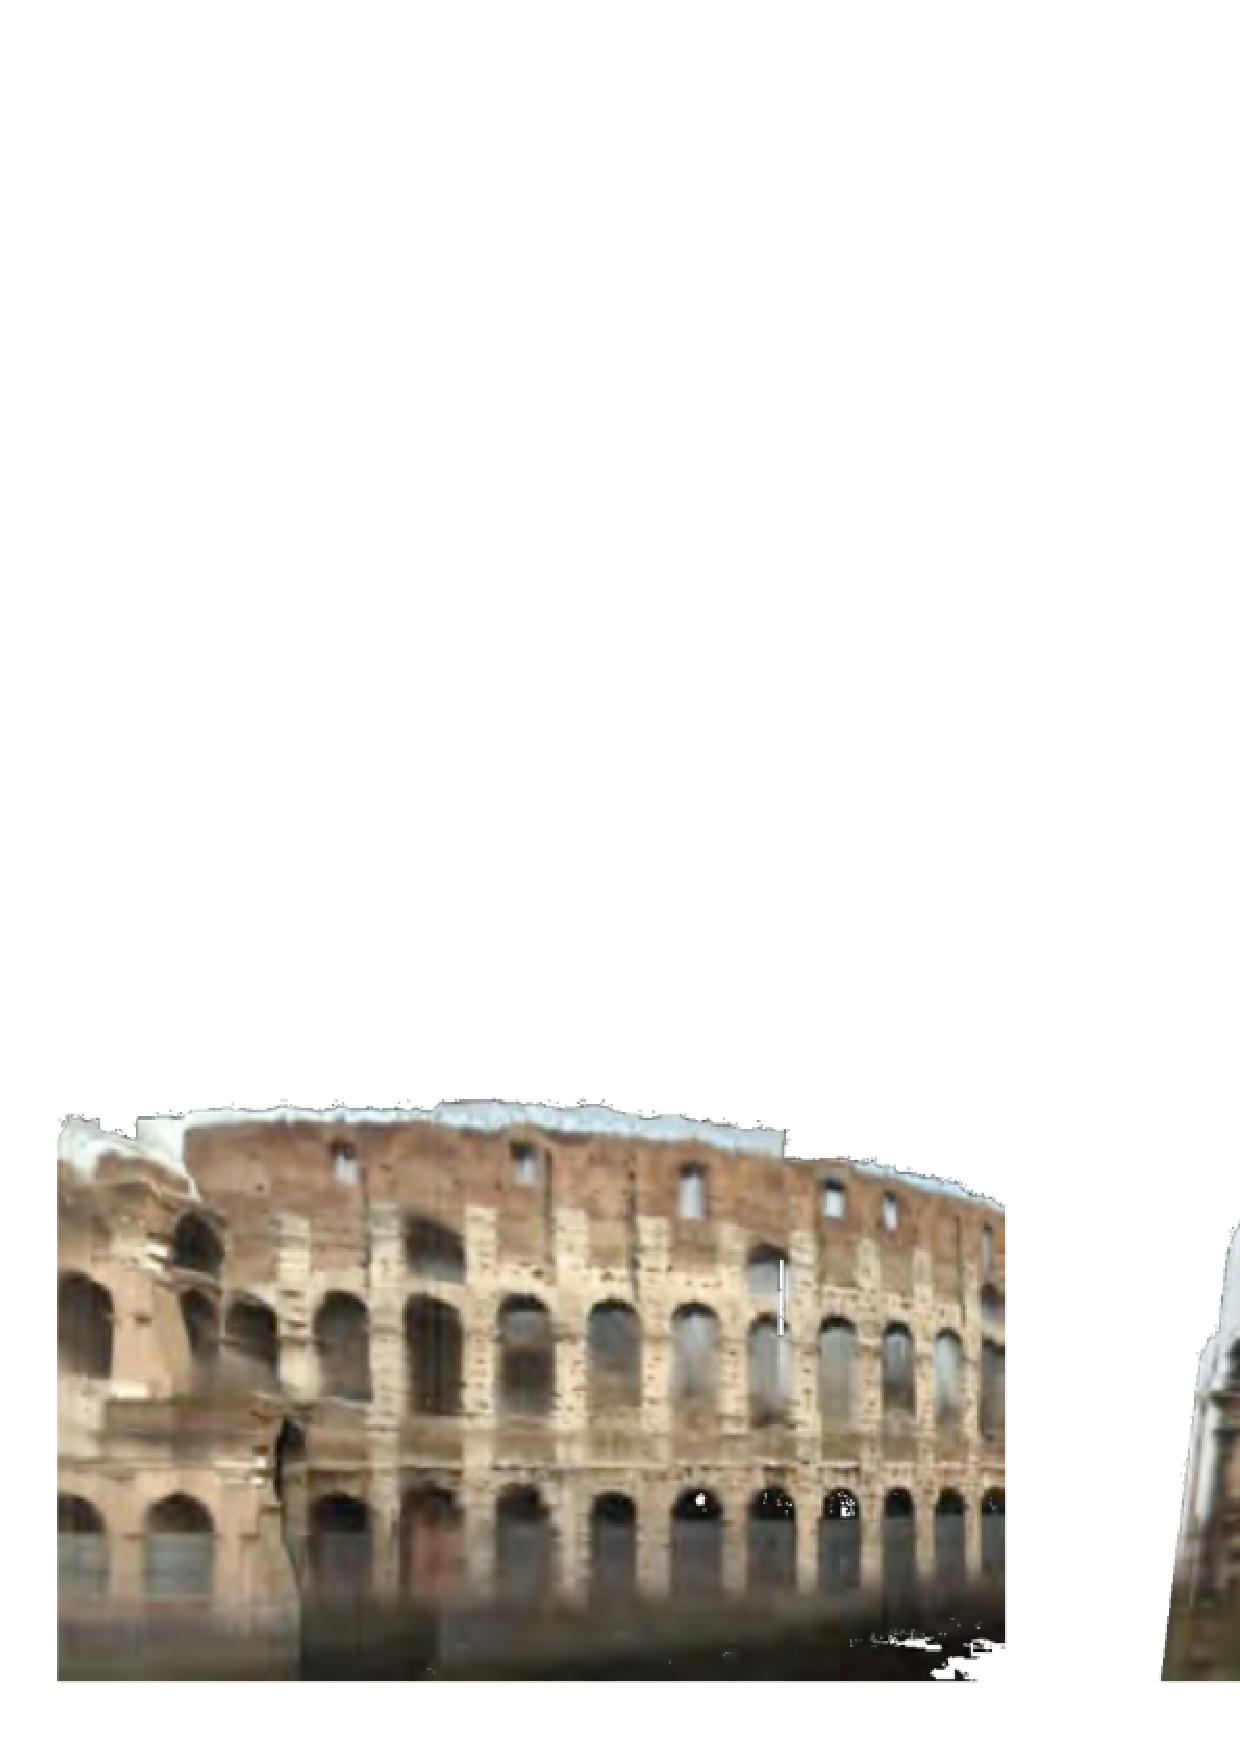
\includegraphics[scale=0.25]{images/jan}
\caption{Reconstructed 3D buildings in less than 24 hr. using 2.8 million and 2.9 million of images respectively}
\label{fig:jan}
\end{center}
\end{figure}

%done
In \cite{guangyu} an hybrid approach is used, combining a ToF (Time of Flight) camera and an grayscale camera in order to perform the reconstruction. 
The data adquisition is made rotating the object in front of the camera with a black background behind it, then they use 
SIFT (Scale Invariant Feature Transform) to find 2D feature correspondences and perform and initial alination between two consecutive frames, this alineation is 
then improved with ICP (Iterative Closest Point) algorithm. They use a 3D laser scanner in order to obtain a ground truth, obtaining a difference around of 1\% 
between their reconstructed
 models and the 3D laser models. See figure \ref{fig:guangyu}.

%put this on the correct place
Its common to find works where the method is not quantitatively evaluated 
in 3D reconstruction due to the high 
cost of a laser scanner that is used as ground truth. 


\begin{figure}[h!]
\begin{center}
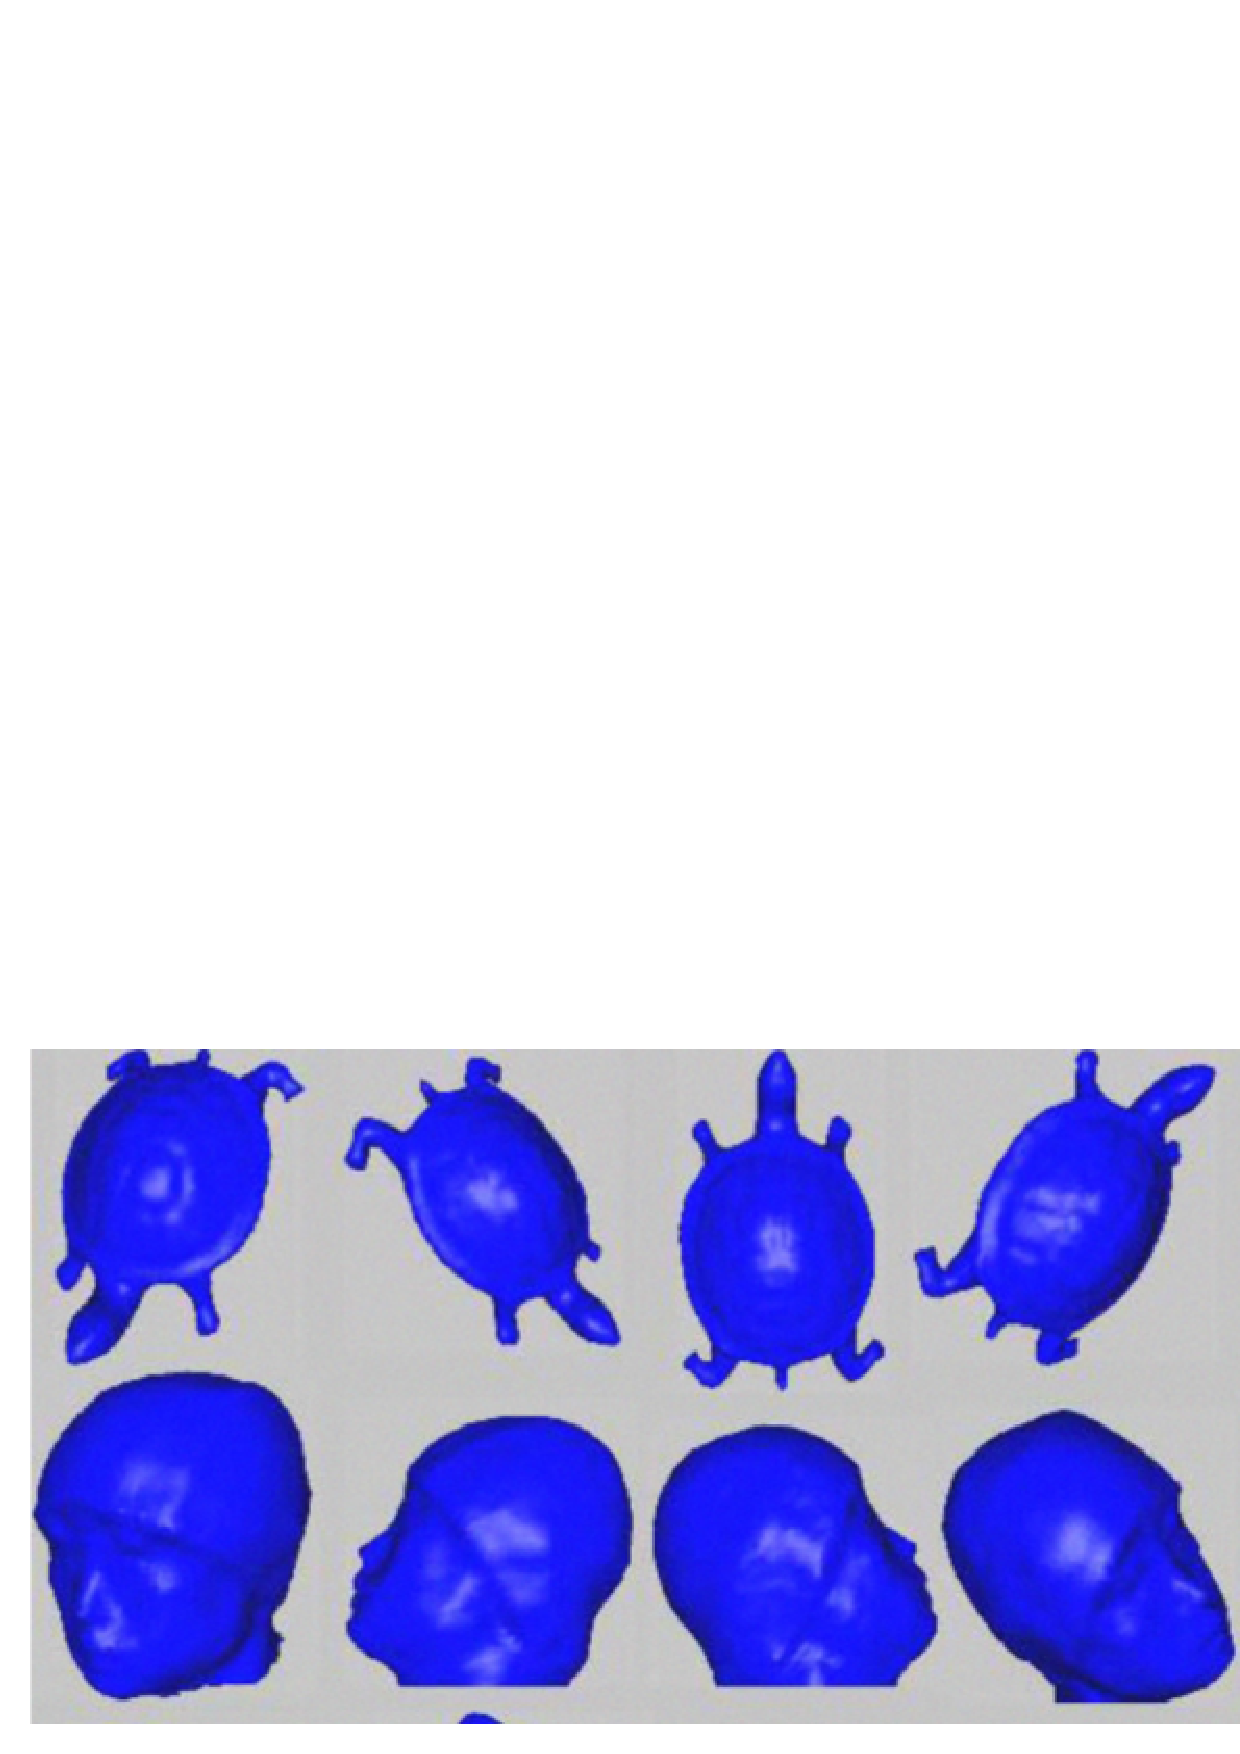
\includegraphics[scale=0.38]{images/guangyu}
\caption{3D Reconstruction of a human head and an object using ToF and RGB camera}
\label{fig:guangyu}
\end{center}
\end{figure}

%done
In \cite{may2009} a ToF camera is used in combination with an industrial robot arm (KUKA KR 16) in order to register an indor scene,
they use an improved version of the ICP algorithm called ICP Frustum, where at each iteration the points that are not overlaping with the previous frame are removed. The industrial robot arm is used to move the camera and get a ground truth camera path to evaluate the performance of their ICP algorithm. 

%Its possible to find more elaborated reconstructions using a laser scanner, but its a more expensive method. In 
%\cite{binney} there is a interesting work where a reconstruction of tree branches is performed using a laser range 
%data. They use a probabilistic approach and use knowledge about the tree structure to guide an iterative reconstruction 
%process. 

%done
In \cite{keqiang} a 3D reconstruction is performed with a laser range finder (SICK 2D ) and a mobile robot, 
using the ICP algorithm and a volumetric representation. In the matching phase of the ICP algorithm not all
 points are used, instead they just use edge points, reducing the computational cost of the process. The scene 
 representation is simplyfied removing redundant points, this is done dividing the scene into voxels and at each 
 voxel preserving just the point closer to the center. Their system produces a scene with data points evenly 
 distributed.

%revisar nuevamente
In \cite{wei} a CCD camera and a 2D laser scanner is used to perform indoor panoramic 3D reconstruction, 
they mounted both devices in a rotational stage and use a fusion algorithm to merge the depth map generated by the laser 
and the depth map generated from the CCD camera observations, the two depth maps contains noise and an intelligent merging reduce this
 noise giving more accurate information to the 3D reconstruction process. Another interesting work of indoor scene reconstruction is \cite{henry} where an RGB-D camera is used to reconstruct an indoor scene. RGB-D cameras are sensing systems that capture RGB images
 along with per pixel depth information. They use the ICP algorithm to calculate the camera location and pass to it information from 
the depth camera and  rich visual
 features along with RANSAC (RAndom SAmple Consensus) verification captured by the RGB camera. They use surfels \cite{pfister} to represent the scene. See figure \ref{fig:henry}.

\begin{figure}[h!]
\begin{center}
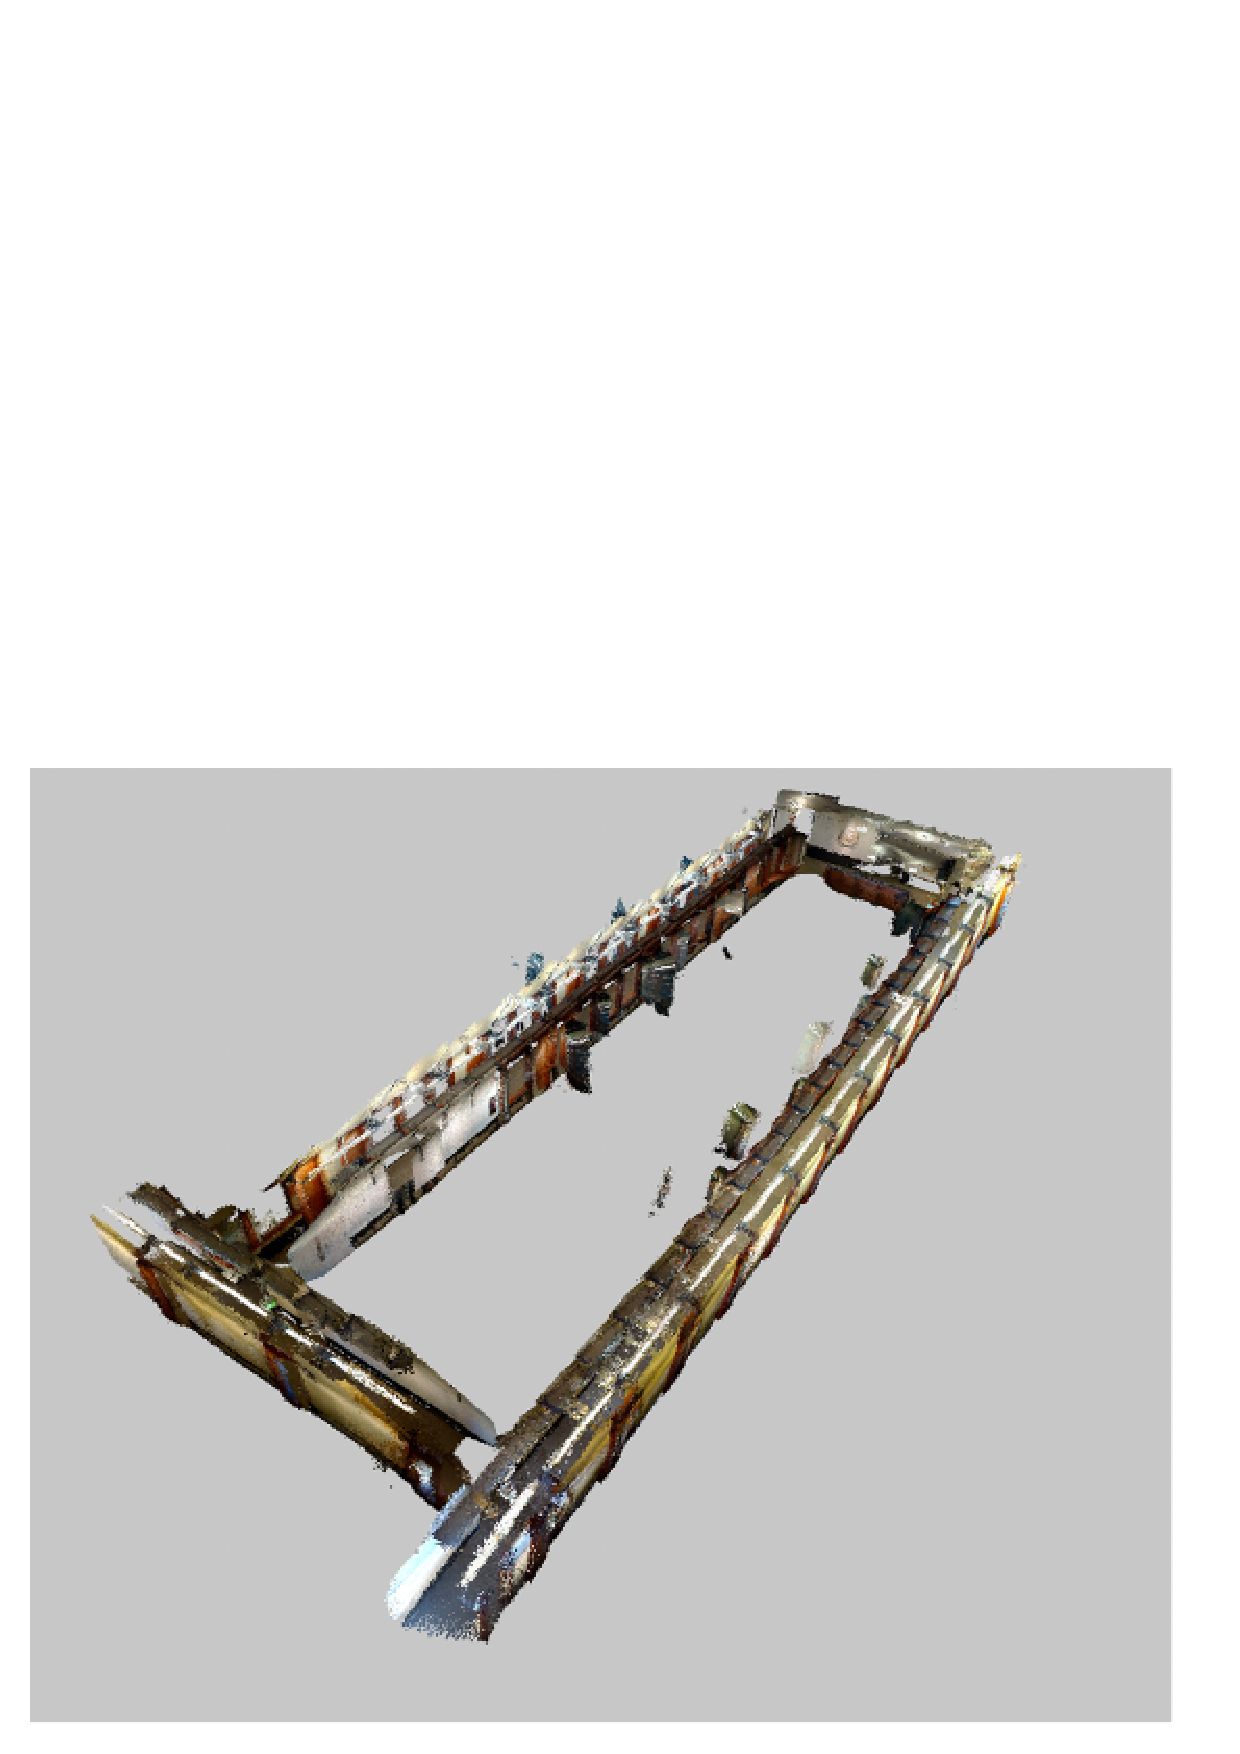
\includegraphics[scale=0.29]{images/henry}
\caption{Reconstructed 3D big indoor space}
\label{fig:henry}
\end{center}
\end{figure}

%done
In \cite{cui} a ToF camera is used to reconstruct 3D objects. A combination of 3D superresolution method with a 
probabilistic scan alignment (iterative Expectation Maximization) approach that takes into account the sensor's 
noise characteristics is used. Their method is not in real time and the resulting models contains undesirable 
artifacts due to  the noise of the captured depth maps, they use a low resolution device (176x144) and they 
improve the resolution using a superresolution method. They captured a ground truth model with a laser 3D scanner, 
obtaining differences below 1 cm in most areas between their model and the ground truth model. Their scanning 
procedure doesn't allow a freely movement around the object, the object must be at the center of view of the camera 
and the distance between the object and camera must be almost constant. A similar work can be found at \cite{schoun} where 
 a hierarchical Lukas Kanade optical flow is used for registration.
 
see figure \ref{fig:cui}.

\begin{figure}[h!]
\begin{center}
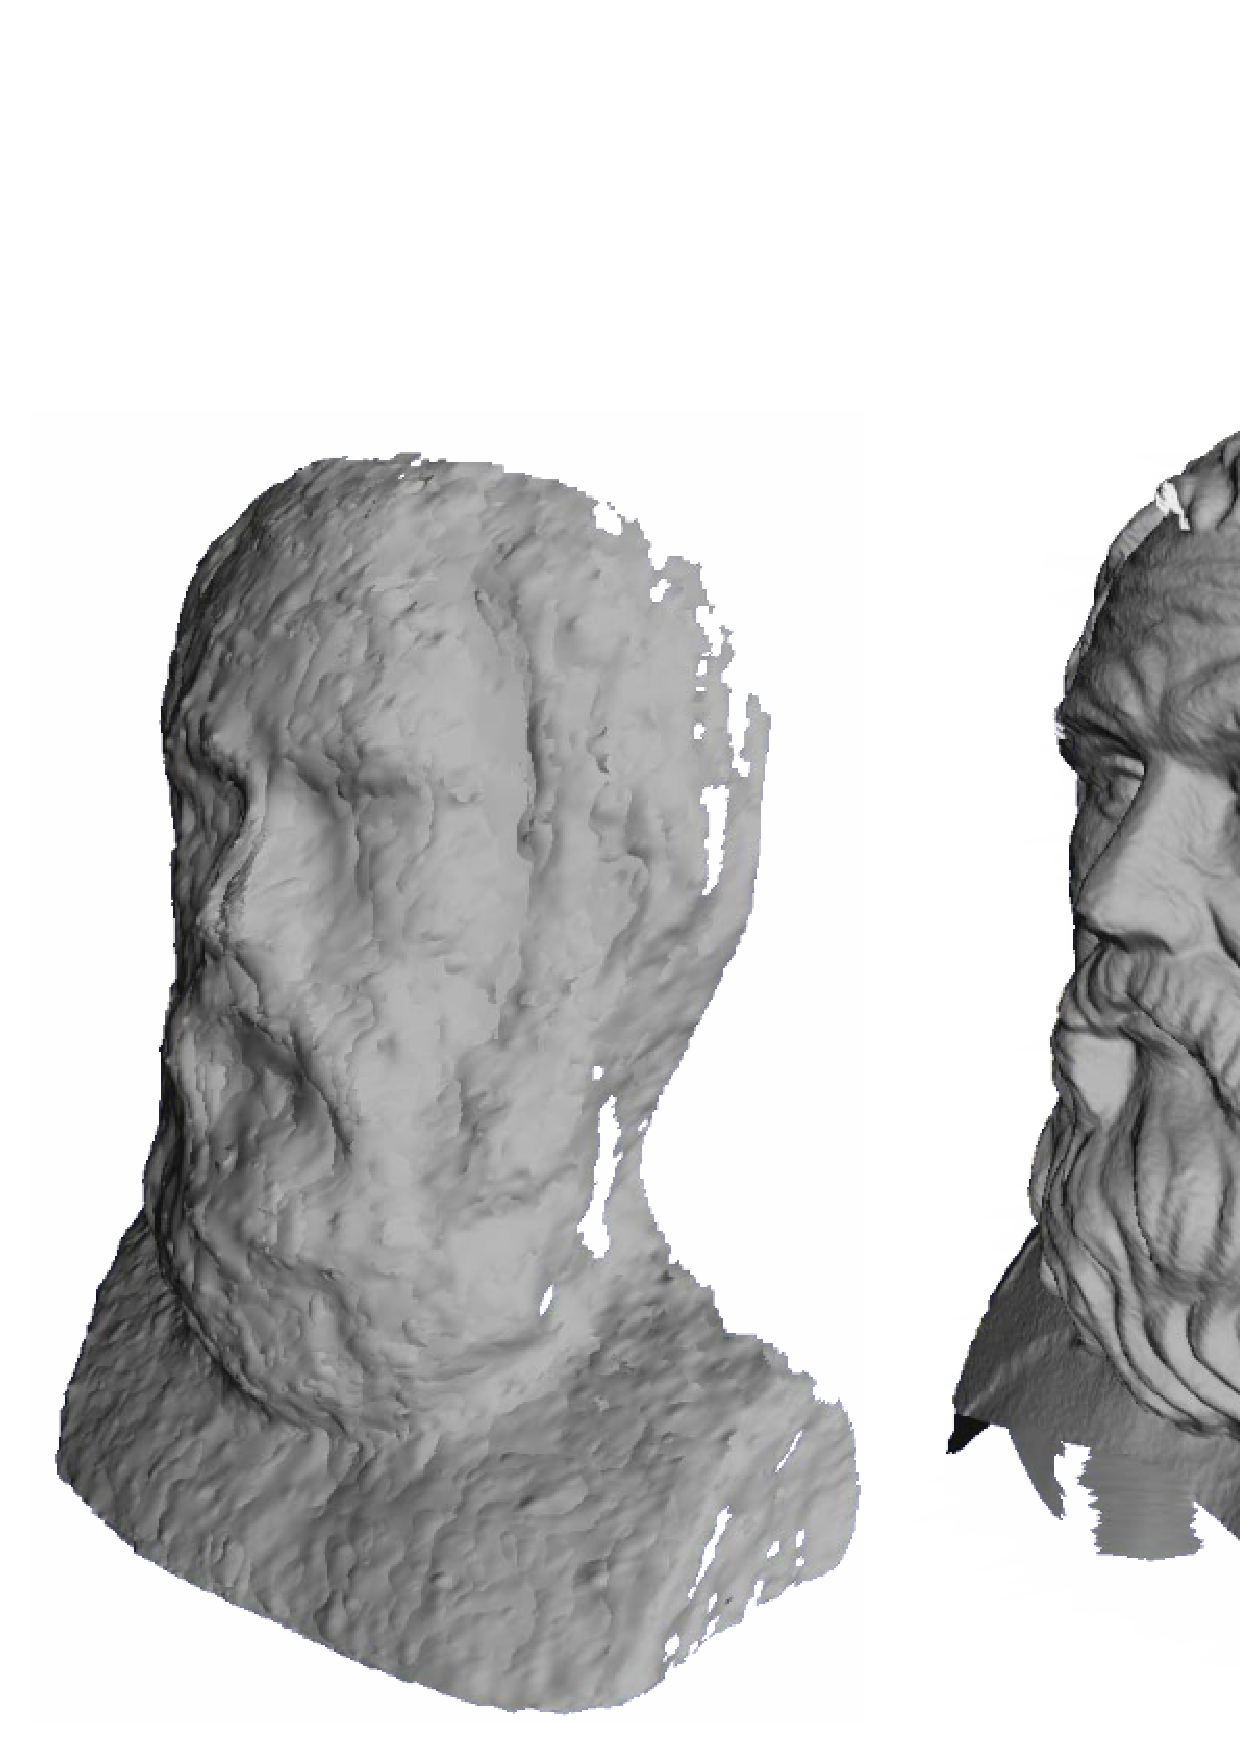
\includegraphics[scale=0.23]{images/cui}
\caption{ToF Reconstruction, Laser Reconstruction and Error Plot}
\label{fig:cui}
\end{center}
\end{figure}

 
%done
A very interesting work is made in \cite{izadi}, they use a low cost RGB-D camera (Kinect) in order to perform
the 3D reconstruction using the ICP algorithm  and a volumetric representation with a GPU in order to 
archieve real time reconstruction. The camera can move freely around the scene and the reconstruction grows in detail 
as new depth measurements are added. They apply color textures to the reconstructed scene obtaining very 
realistic models, their system is able to perform rigid body collisions 
simulations during the reconstruction, allowing thousands of virtual particles interact with the scene. Also a 
user can interact with the scene during the reconstruction process. This is one of the most advanced 
reconstruction systems, due to its uniques features.

 see figure \ref{fig:izadi}.

\begin{figure}[h!]
\begin{center}
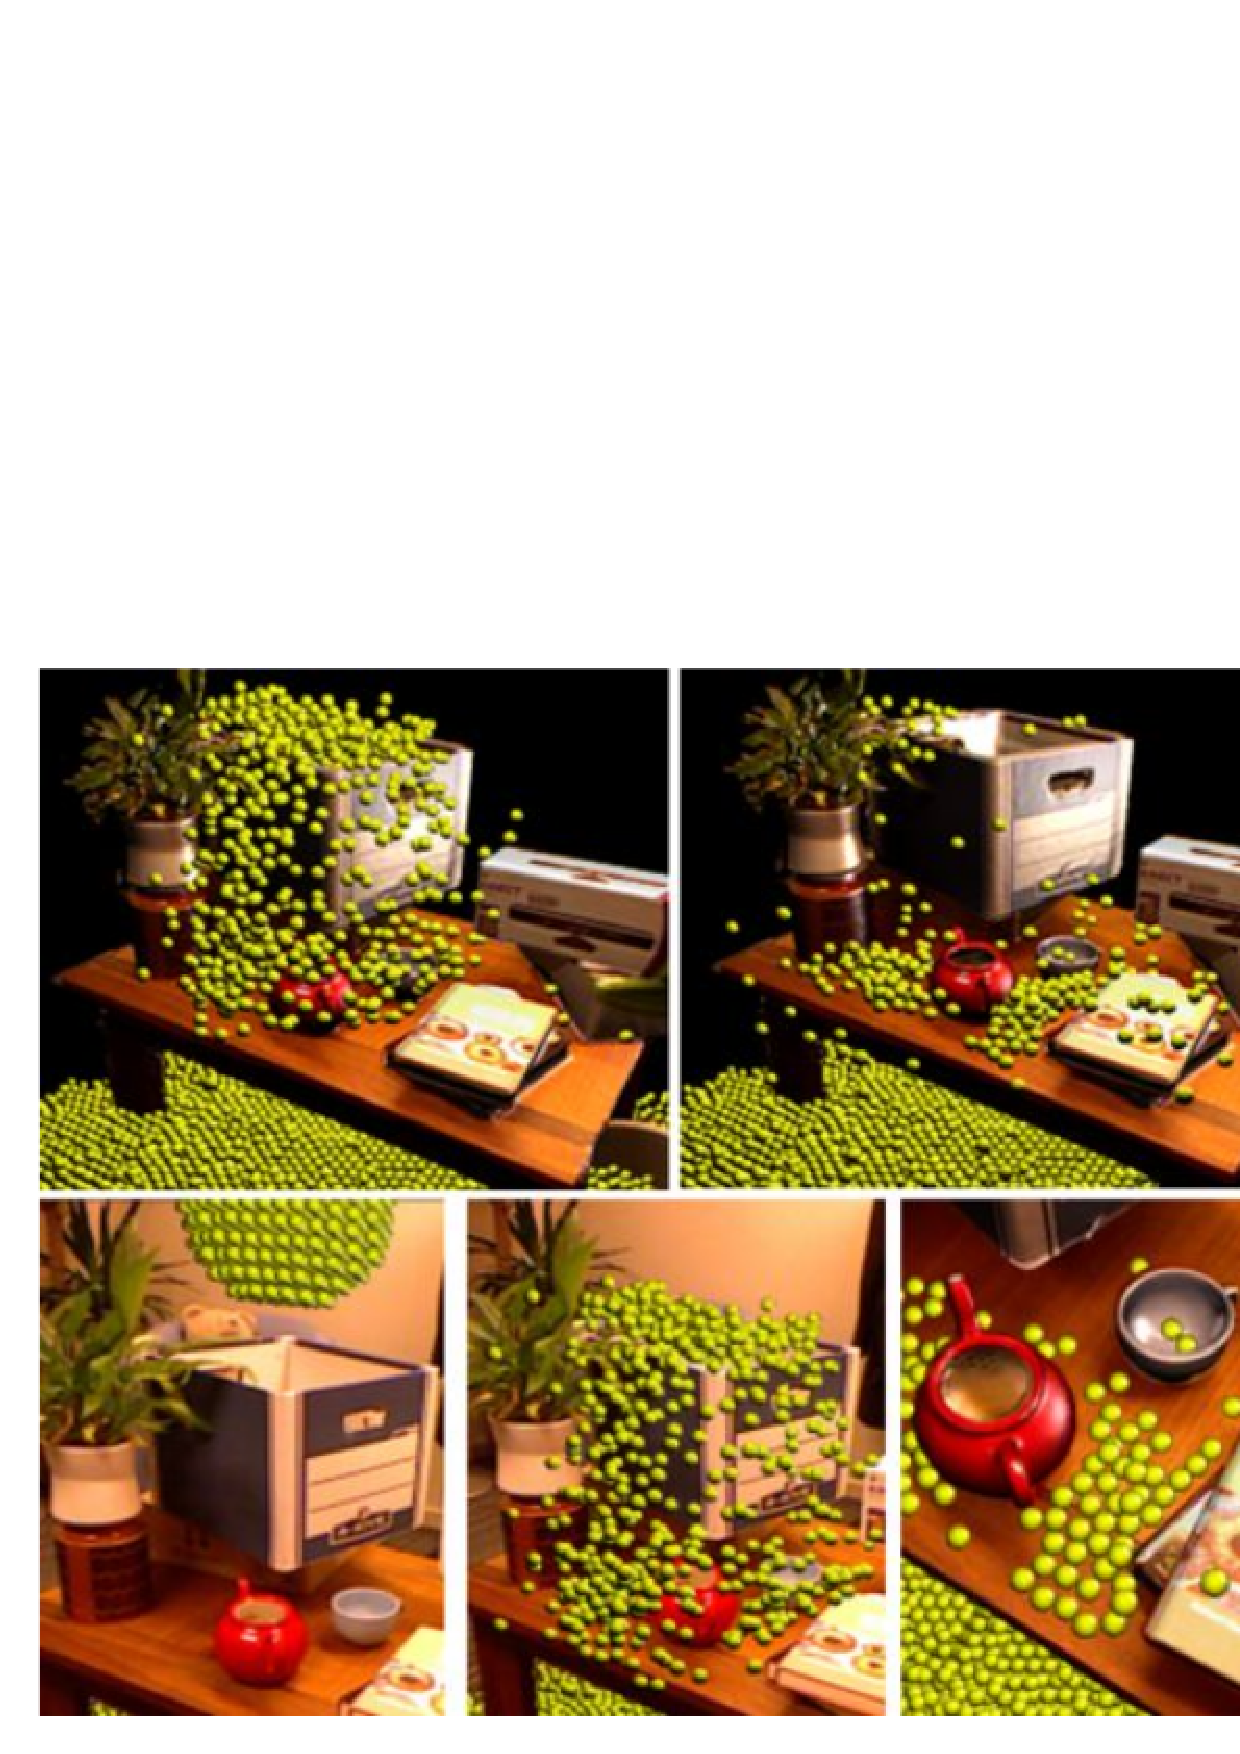
\includegraphics[scale=0.34]{images/izadi}
\caption{Reconstructed 3D scene with thousands of virtual particles}
\label{fig:izadi}
\end{center}
\end{figure}


All the 3D reconstruction methods can have problems with non lambertian 
surfaces and they need to make some assumptions about the surfaces reflectance. For example if we are using 
an infrared structured light pattern depth camera and the object that we are registering absorbs the infrared light, 
the reconstruction will fail. Similar problems can occur with laser scanners. 
Some materials such as glass or water can ruin the reconstruction.


%must be correctly located
In \cite{weise08} the user move the object using his hands in front of an RGB-D sensor (In-hand modeling), the hands are 
eliminated using a color skin detector and the user can see the reconstruction in real time, in order to correctly 
move the object.  The object is registered with Fast ICP, which instead of searching for the closest 
point, projects a transformated source point on the 2D target depth image in order to perform the matching. They use point
 to plane distance. This ICP variation is also used in \cite{jaeggli03}. \cite{weise08} uses geometrical and visual 
information to perform a correct registration. Imposing geometrical contraints based on the cameras lines of sight and visual 
contraints applying Gaussian derivative kernels to both images and measuring similarities.







\chapter{Sensor}
\index{Sensor}

\section{Pinhole Camera Model}

The pinhole camera model describes the mathematical relationship between the points of the image plane and the 3D points captured by an 
ideal pinhole camera. In the context of this work, this model is useful to explain how the depth is calculated by Kinect and 
how to reproject points in the photoconsistency method.

\begin{figure}[H]
\begin{center}
\includegraphics[scale=0.15]{images/pinhole-camera}
\caption{Pinhole camera}
\label{fig:pinhole}
\end{center}
\end{figure}

In the pinhole camera all rays pass from the scene to a photosensitive material through a pinhole, in order to form the image.

\begin{figure}[H]
\begin{center}
\includegraphics[scale=1]{images/pinhole-coordinates}
\caption{Pinhole camera coordinates system}
\label{fig:pinhole-c}
\end{center}
\end{figure}

In \ref{fig:pinhole-c} the point P denotes the principal point, O is the optical center and 
f=dist(P,O) is the focal lenght.

The transformation between world coordinates point (X,Y,Z) and image coordinates (x,y) is described as 
follows:

\begin{equation}
\label{eq:disparity2}
 x = \frac{fX}{Z},
\end{equation}

\begin{equation}
\label{eq:disparity2}
 y = \frac{fY}{Z}.
\end{equation}

These equations are  obtained using triangles similarity.

\section{Kinect Sensor}

Kinect sensor was launched at the end of 2010 by Microsoft. A structured light camera 
used as peripheral for the Xbox 360. With solds of more than 24 million devices at february 2013.
The sensor gained great attention from computer vision and robotics communities, because it offers 
accurate depth information at low cost in comparison to existing alternatives.

\section{Sensor Depth Calculation}

The Kinect sensor consists of an infrared laser emitter, an 
infrared camera and an RGB camera. Both cameras can work up to 30Hz. 
The laser source emits a single 
beam which is split into multiple beams by a diffraction 
grating to create a constant 
pattern of speckles projected onto the scene. This pattern is 
captured by the infrared camera and is correlated against a 
reference pattern. The reference pattern is obtained by capturing 
a plane at a known distance from the sensor, and is stored in the 
memory of the sensor. When a speckle is projected on an object 
whose distance to the sensor is smaller or larger than that of the 
reference plane the position of the speckle in the infrared image 
will be shifted in the direction of the baseline between the laser 
projector and the perspective centre of the infrared camera. 
These shifts are measured for all speckles by a simple image 
correlation procedure, which yields a disparity image \cite{khoshelham2011accuracy} . For each 
pixel the distance to the sensor can then be retrieved from the 
corresponding disparity.



\begin{figure}[h!]
\begin{center}
\includegraphics[scale=1.65]{images/kinect_triangulation}
\caption{Schematic representation of depth-disparity relation. Image taken from \cite{khoshelham2011accuracy}}
\label{fig:disparity}
\end{center}
\end{figure}

\begin{equation}
\label{eq:disparity1}
 \frac{D}{b} = \frac{Z_0 - Z_k}{Z_0},
\end{equation}


\begin{equation}
\label{eq:disparity2}
 \frac{d}{f} = \frac{D}{Z_k}. 
\end{equation}

Then $Z_k$ can be obtained from \ref{eq:disparity1} and \ref{eq:disparity2}. Where variables $Z_0$,$b$ and $f$ are known.

\section{Sensor Captured Data}
\label{sec:sensor_data}

The sensor obtains two images: An RGB color image and a depth map. 

The RGB color image has three channels: Red, Green and Blue. And each image color is generated 
combining this three colors. With a resolution of 640x480 pixels and 1 byte per channel. The sensor can 
capture color images at higher resolutions, but in our case we need just one color per depth map pixel.

The depth map is like a gray scale image where the value of each pixel is the object distance to the sensor in the viewing axis. 
The depth map is an image with a resolution of 640x480 and one channel of 2 bytes. We use meters as distance unit.

\begin{figure}[h!]
\begin{center}
\includegraphics[scale=0.3]{images/color_depth.png}
\caption{Left: RGB image, right: depth map converted to a grayscale image (0-255 values) for visualization purposes}
\label{fig:colordepth}
\end{center}
\end{figure}


\begin{figure}[h!]
\begin{center}
\includegraphics[scale=0.25]{images/3d_point_cloud.png}
\caption{Different perspectives of 3D color point cloud obtained combining the RGB image colors and the depth map 3D points}
\label{fig:colorpcloud}
\end{center}
\end{figure}


The depth map implicity contains the objects world coordinates, the relation between depth map 
and world coordinates is described as follows:

\begin{equation}
\label{eq:depthmapx}
 X=\frac{(x-x')Z}{f},
\end{equation}

\begin{equation}
\label{eq:depthmapy}
 Y=\frac{(y-y')Z}{f}.
\end{equation}


\noindent Where $(x',y')$ is the image principal point (projection of optical center on the image plane), f is the camera 
focal length, $(x,y)$ are the 2D coordinates in the depth map plane (640 pixels width, 480 pixels height) and $Z$ is the distance in the viewing axis from the camera to the object that is in position $(x,y)$ of depth map.

\begin{figure}[H]
\begin{center}
\includegraphics[scale=0.55]{images/coordinates}
\caption{Kinect coordinates system}
\label{fig:coordinates}
\end{center}
\end{figure}

In this work we will use the RGB image, the depth map and the point cloud obtained combining both.
 
The RGB camera has a slightly larger angle of view than the depth camera, for this reason a calibration must be done 
in order to have RGB images and depth maps using the same coordinates. The dataset already has RGB images and depth maps 
calibrated. More information about 
this process can be found in \cite{sturm12iros}.


\chapter{Proposal}
\index{Proposal}
One of the first fundamental steps to reconstruct a 3D scene is the 
positioning of the 3D points on a common coordinate system, conserving 
the original scene structure. This step is called registration. 

In general, when the sensor is collecting the 3D points from the scene, 
 its necessary to move or rotate it in order to capture new objects and surfaces from 
the scene, adding more information to the reconstructed scene. But in order to be 
able to infer the correct position of each capture, is necessary to have part 
of the view in common between two captures (an overlaping area). Thus is posible 
to position a new capture with respect to an old one in the scene, using this overlaping 
area to correctly align both captures.
 
The overlaping areas of the different captures of a scene must be correctly 
aligned when registering the points in a common coordinate system, 
thus with each new capture more information is added to the scene, 
getting closer to the desired result. 

The most used algorithm for solve this problem is called 
ICP (Iterative Closest Point) Algorithm. Given two point clouds, 
this algorithm find the best rigid transformation to align both clouds 
(minimize distance between puntos emparejados). In order to make this, 
the algorithm starts with an initial guess of the transformation. 
At each iteration the algorithm matchs points of each cloud and then 
find the best transformation. 





\section{Bilateral Filter}


The depthmaps captured by a low cost RGB-D camera usually contains noise, this can be 
consecuence of materials reflectance, device imperfections, object fast movement, distance to the 
sensor, etc. 

In order to reduce the effect of noise is natural to use some kind of filter, as usual in computer 
vision, a typical filter will take information of a pixel and its neighboorhod to generate a result. 
If the image is smooth, without abrupt changes in intensity, a simple average could be enough. However, this 
is not the case in the presence of edges or corners, areas where the intensity changes charply. 
The bilateral filter afronts this problem, giving to each neighboor a weight based on its cercany  
to the center pixel. In a grayscale image it takes into account 
the neighboor intensity distance and location distance (in image plane) to calculate the weight.  A depthmap is very similar to a grayscale 
image, the only difference is that the depth map represents geometrical information and usually contains holes 
(areas where the sensor failed to capture distance). 

A bileateral filter was applied to the depth maps, using the euclidean distance and the distance along the z axis to calculate 
the weight of each pixel neighboor in the depth map.

In a filter window centered at pixel location $(x,y)$, the weighted average was calculated using the following weight for each neighboor:


$$ w(p,q,\sigma_d,\sigma_z) = k(d(p,q),\sigma_d) k(z(p,q),\sigma_z). $$

\noindent Where 

$$ k(v,\sigma) = \frac{e^{-v^2}}{2*\sigma^2}, $$
$$ d(p,q) = ||p - q||, $$
$$ z(p,q) = |p_z - q_z|, $$
$$ p = (p_x,p_y,p_z), $$ 
$$ q = (q_x,q_y,q_z). $$

\noindent p is the central point 3D coordinate and q the 3D coordinate of one of its neighboors. 3D coordinates are obtained using
 the depth map and equations \ref{eq:depthmapx} and \ref{eq:depthmapy}.  Each point has a weight that depends on its euclidean distance and
 the distance along the z axis, to the central point. The parameter $\sigma_d$ defines 
the neighborhood, all points of the depthmap that are at euclidean distance $2*\sigma_d$ or less from the central pixel are considered.


Let 


$$ W = \sum\limits_{q \in neighborhood} {w(d,\sigma_d,z,\sigma_z)},$$

\noindent the final value of the center pixel is then

$$p_z = \frac{1}{W}\sum\limits_{q \in neighborhood}{w(d,\sigma_d,z,\sigma_z)p_z}.$$

\noindent where the neighborhood is conformed by the points at an euclidean distance less than $2*\sigma_d$.

After applying this filter we obtain an smoothed version of the depth map, without loosing edges and important geometrical information.
A detailed explanation of the bilateral filter can be found in \cite{TomasiBilateral}.

\begin{figure}[h!]
\begin{center}
\includegraphics[scale=0.35]{images/bilateral}
\end{center}
\caption{Left: Point cloud without filtering Right: Point cloud with bilateral filtering. Noticeable effects at first sight next to the borders of objects}
\end{figure}


\section{Borders Filter}

Edges are widely used in computer vision, they contain rich information about texture 
and geometry, for this reason edges are features that are usefull for several tasks, 
such as object recognition, object traking, etc.


The Sobel filter is a wellknown edge detector. To apply this filter is necessary to 
convolve the image with two 3x3 matrix, to find intensity changes in vertical and 
horizontal directions:

\begin{center}
\includegraphics[scale=0.35]{images/sobel}
\end{center}

Then both results are merged using the bellow expression and then a threshold is used to filter out non interest areas:

$$ G = \sqrt{G_x^2+ G_y^2} $$

This filter is applied directly into a grayscale representation of the original RGB image. Obtaining a binary image 
that contains edges, not necessarily corresponding to intensity changes, that can occur as consecuence of both, geometrical 
and visual changes in the scene.

%edges image

This image can be used along with the depth map to reduce the point cloud size. Rejecting all 3D points not corresponding
to this edges. We are interested in find correspondences between the two clouds, for this reason, we applied the edge filtering 
to the image instead of the depthmap. Because using this approach it is possible to find corresponcendes between rich textured 
surfaces, even if they don't exhibit geometrical richness.

This filter is applied to both, source and target captures. Making this, it is possible to apply a very useful filtering: remove 
from the edges binary image all the points that are not simultaneously in both captures. For this, the rotation and translation 
of the source 2D image that minimizes the distance to the target 2D image is applied and then an AND operation is applied between 
the two images. As result, we work with two point clouds that have a huge amount of overlaping points, improving the alineation 
result.


A Sobel filter was used to obtain a representative set of points, avoiding that walls and another 
plain surfaces containing a huge amount of data, lead to an incorrect alineation.

\begin{figure}[h!]
\begin{center}
\includegraphics[scale=0.35]{images/sobel_v_h.png}
\caption{Left: Sobel vertical filtered point cloud, Right: Sobel horizontal filtered point cloud}
\end{center}

\begin{center}
\includegraphics[scale=0.35]{images/sobel_o_g.png}
\caption{Left: Original point cloud, Right: Sobel filtered point cloud}
\end{center}
\end{figure}

There are more advanced edge filtering techniques, such as the Canny edge filter, but it involve 
a larger set of convolutions and operations. We dont need an high accuracy edge detection, the Sobel 
filter is enough to reduce the set of points used in the alineation process.


 


There are several techniques to track an object. If there is information about the object of interest the problem 
can be simplyfied using this information to restrict the search space, for example to certain color or shape.
 By the other hand if the object to track is unknown, it is necessary to find a more general feature, that is 
more likely to be found on the unknown interest objects. The corners are good features for this purpose. A corner 
is a point on the image where there are gradient variations on two orthogonal directions.

The most common definition of a corner is gived by Harris :

$$
E(u,v) = \begin{bmatrix} u & v \end{bmatrix} \sum\limits_{x,y} w(x,y) \begin{bmatrix} {I_x}^2 & I_x I_y \\ I_x I_y & {I_y}^2 \end{bmatrix} \begin{bmatrix} u \\ v \end{bmatrix}
$$

We loop over a neighboorhood defined by different values of (x,y) and calculate 
the difference of each pixel located at (x,y) with some other pixel located at (x+u,y+v). 
The function w(x,y) is used to give some weight to each pixel. 


Optical Flow

The optical flow methods are used to calculate motion between two sucesive image frames which are taken
 at two different times: t and \delta t.

This methods have three main supositions about the frames:

1.- The intensity remains constant
2.- They are geometricaly consistent
3.- There is a rigid transformation between one frame and the next

There are two kinds of optical flow: dense and sparse. Dense optical flow means  calculate direction vector for each pixel of the image and sparse optical flow is calculate direction vector just those pixels of the image 
who satisfy certain conditions.

Dense optical flow is computationally expensive and its difficult to find the direction vector for plain color areas. For example an image of a white paper, there are a lot of pixels with the same properties and its necesary to perform some kind of interpolation to lidiar with this pixels. By the other hand, sparse optical flow just consider pixels with more odds of been matched between the two frames.





\section{Photoconsistency}

Having a estimation of rotation R and translation t, it is possible to reproject the 3D points to the 2D image plane using the 
camera parameters. If we have a point $p=(X,Y,Z)$ we can project it to the image plane using the following formula obtained 
from the pinhole camera model:

\begin{equation}
U(p) = (\frac{fX}{Z} - c_x, \frac{fY}{Z} - cy)
\label{eq:reproject}
\end{equation}

Where $f$ and $(cx,cy)$ denote the focal length and optical center of the pinhole camera model. 
We can apply the transformation R,t to the point before projecting it:

\begin{equation}
T(R,t,p) = Rp + t = p'
\end{equation}

Image coordinates  $p'$ are used to obtain image color in the target image, making a reprojection of $p'$ to the image plane.

Then we can apply the following error formula, that represents the color differences between the reprojected image and 
the target image. 

\begin{equation}
E(R,t) = \frac{1}{N} \sum\limits_{p \in pointCloudSource} |RGBsource(U(p)) - RGBtarget(U(p'))|
\end{equation}


Where:
\begin{itemize}
\item N is the number of points.
\item $U(p)$ is the reprojection function \ref{eq:reproject} that returns (x,y) image coordinates of an (X,Y,Z) point.
\item  $RGBsource(x,y)$ is function that returns a vector (R,G,B) representing image color at location (x,y). Where 
R,G,B are positive integers between 0 and 255. The same holds for $RGBtarget(x,y)$. Both functions represent 
source and target images respectively.
\end{itemize}

In this case the average color difference vector norm is used, but there are many ways of measure photoconsistency, 
for example using a color space different from RGB or using another error metric. Photoconsistency is widely used in 3D reconstuction, for example some works using it are \cite{Whelan13},\cite{kerl13icra} and \cite{Newcombe10livedense}



\section{Iterative Closest Point}

The ICP (Iterative Closest Point) algorithm \cite{mckay92} is widely used for 3D Reconstruction. This algorithm tries to find 
the optimal rotation and translation between two sets of points (point clouds) that minimizes the distance between corresponding 
points. Corresponding points are determined assigning to each point of one cloud, the closest point in the other cloud.

As result at each iteration we have a set of pairs of closest points, where each pair contains one point of each cloud. This set 
of pairs changes from iteration to iteration, since the rotation and translation updates the points of one of the point clouds. If enough correct 
corresponding points are find in each iteration, the algorithm converges to the correct transformation that aligns both point clouds.


%\tiny
R : 3x3 Rotation matrix

t : 3x1 Translation vector

A,A',B : Point sets $\in R^3$

p : Pair set

%\small
\begin{algorithm}
\caption{ICP algorithm}
\begin{algorithmic}[1]
\State init(R,t)
\State A' $\leftarrow$ transform(A,R,t) 
\State p $\leftarrow$ closestPoints(A',B)
\State $\{R,t\} \gets$ updateTransformation(p)
\State $e_i = meanSquareError(p)$
\If {$e_i < umbral$ OR  $i > maxIteracions$} 
	\State return R,t
\Else
	\State go to step 2
\EndIf
\end{algorithmic}
\end{algorithm}


We want to find R and t that minimizes the following expression:

$$ \sum\limits_{i=1}^n ||R a_i -  b_i - t ||^2 $$

Where each $a_i,b_i$ is a vector $\in \mathbb{R}^3$, R is a 3x3 rotation matrix and t is a vector $\in \mathbb{R}^3$


We make a change of coordinates, placing the centroid of each cloud as origin:



\begin{align*}
 \bar{a} = \frac{1}{n} \sum\limits_{i=1}^n {a_i} \\ 
  \bar{b} = \frac{1}{n} \sum\limits_{i=1}^n {b_i} \\  
   {a'}_i = a_i - \bar{a}\\
   {b'}_i = b_i - \bar{b} 
\end{align*}

Replacing

\[ \sum\limits_{i=1}^n ||R a_i -  b_i - t ||^2 = \sum\limits_{i=1}^n ||R ( {a'}_i + \bar{a} ) -  ( {b'}_i  + \bar{b} ) - t ||^2  \]

The desired translation is $t = R \bar{a} - \bar{b} $. We must consider the rotation in this expression, since 
the rotation of a cloud will change the position of all points and as consecuence the translation.

Replacing t in our previous expression we get:
\begin{flalign*}
&\sum\limits_{i=1}^n ||R a'_i - b'_i ||^2  \\ 
&=\sum\limits_{i=1}^n (R a'_i - b'_i)^t (R a'_i - b'_i) \\
&=\sum\limits_{i=1}^n ( (R a'_i)^t R a'_i - (R a'_i)^t b'_i  - b_i^{\prime t} R a'_i + b_i^{\prime t} b'_i) \\
&=\sum\limits_{i=1}^n ( a_i^{\prime t} R^t R a'_i - 2 b_i^{\prime t} R a'_i + b_i^{\prime t} b'_i) \\ 
&=\sum\limits_{i=1}^n (a_i^{\prime t} a'_i -  2 b_i^{\prime t} R a'_i + b_i^{\prime t} b'_i) 
\end{flalign*}


Minimize the previous expression is equivalent to maximize:

\begin{align*}
& \sum\limits_{i=1}^n b_i^{\prime t} R a'_i =  Trace ( \sum\limits_{i=1}^n R a'_i  b_i^{\prime t} ) = Trace (RH) \\
& H=\sum\limits_{i=1}^n a'_i  b_i^{\prime t} 
\end{align*}


\begin{mybox}{gray}{Lemma}
For any positive definite matrix $A A^t$ and any orthogonal matrix B 

\[ Trace( A A^t ) \geq Trace (B A A^t) \]

\end{mybox}


Proof of lemma:

Let $a_i$ be the ith column of A, then:

\begin{align*}
Trace( B A A^t ) = Trace (A^t B A) = \sum\limits_i a_i^t B a_i 
\end{align*}

But by the Schwarz inequality

\[ a_i^t B a_i \leq \sqrt{ a_i^t a_i (a^t B^t B a_i)} = a^t a_i \]


Now using this lema we will maximize our expression:


Lets apply the SVD factorization to H, then:

\[ H = U \Sigma V^t \]

Where U and V are 3x3 orthonormal matrices and $\Sigma$ is a diagonal matrix with no negative elements.

Let $ R = V U^t $ then :

\begin{align*}
RH = VU^t U \Sigma V^t = V \Sigma V^t = V \Sigma^{\frac{1}{2}} (V \Sigma^{\frac{1}{2}})^t
\end{align*}

Which is symetrical and positive definite.
Therefore from Lemma, for any 3x3 orthonormal matrix B

\[ Trace( R H ) \geq Trace( B R H ) \]

Thus the solution for our problem is 

\begin{align*}
R = V U^t \\
t = R \bar{a} - \bar{b}
\end{align*}


This means that if we apply the rotation R and the translation t, to each point of the point cloud A, the distance between closest points of 
transformed point cloud A with point cloud B will be minimal. When registering a set of points from a real 3D scene it allows to obtain a correct 
align between sucesive scene captures.

\section{Pose Graph Optimization}
\label{sec:posegraph}
When the amount of registered frames increments, the accumulated error 
becomes visible. There is a drift respect to the real sensor trajectory. 
In order to deal with this problem, the most common approach is to use a pose graph 
optimization algorithm. 


Each pose of the sensor (rotation and translation) represents a node of the 
graph and each restriction between two poses represents an edge. The relative 
transformation between two poses is used as restriction.


The first pose of the graph can be arbitrary, in our case is set as the identity. Subsequent 
poses are determined by using relative transformations between pairs of frames, applying 
proposed technique. Each sensor frame corresponds to a graph pose. 

We have a non-linear least squares minimization problem that can be described by the following equation:

$$ F(x) = \sum\limits_{<i,j> \in C } e(x_i,x_j,z_{ij})^T \Omega_{ij} e(x_i,x_j,z_{ij}) $$

$$ x^* = \mathop{\rm argmin}_x F(x) \ ,$$

\noindent where $x=\{x_1,x_2,...,x_n\}$ and each $x_i$ represents a parameter block , $z_{i,j}$ and $\Omega_{ij}$ represents the mean  
 and the information matrix  of a constraint 
relating parameters $x_i$ and $x_j$. In our case $x_i$ corresponds to a sensor pose, $z_{ij}$ is the 
relative transformation between $i$-$esim$ and $j$-$esim$ sensor frame, it is not affected by the accumulated error 
because it is a direct measure between the two frames and $\Omega_{ij}$ is the weight or 
the confidence we give to the restriction. $\Omega_{ij}$ is a $7\times7$ diagonal matrix, containing on its diagonal the confidence ($\in [0,1]$) for each 
parameter of the transformation. 

Poses and relative transformations are represented by a $7\times1$ vector containing a translation vector
 and a normalized quaternion for the rotation:

$$ \begin{bmatrix} tx & ty & tz & qx & qy & qz & qw \end{bmatrix} ^T \ .$$



Then $e_{ij}$ is an error vector ($7\times1$) defined as follows:

$$
e(x_i,x_j,z_{ij}) = z_{ij} - \hat{z_{ij}} \ ,
$$

\noindent where $\hat{z_{ij}}$ is the relative transformation between $x_i$ and $x_j$ obtained directly from the pose graph, for this reason 
it is affected by the accumulated error.

We want to find a graph configuration (updating the poses $x=\{x_1,x_2,...,x_n\}$), that reduces global error,
 correcting some poses in order to satisfy the restrictions.

This  non-linear least squares problem can be solved using 
methods such as for example Gauss-Newton or Levenberg-Marquardt.

\begin{figure}[!h]
\begin{center}
\includegraphics[scale=1.5]{images/graph_diagram2}
\caption{Graph of poses $(x_1,x_2,..)$ with constraints $(z_{12},z_{23},...)$ relating poses.}
\end{center}
\end{figure}

To simplify notation let: 

$$
e(x_i,x_j,z_{ij}) = e(x_i,x_j) = e_{ij}(x) \ ,
$$

\noindent we can approximate the previous function around one point:

\begin{equation}
\label{eq:errorAprox}
e_{ij}(x + \Delta x) \simeq e_{ij}(x) + J_{ij} \Delta x \ ,
\end{equation}

\noindent $J_{ij}$ is the Jacobian of the function evaluated in x. 


\begin{equation}
\label{eq:globalFunc}
F_{ij}(x + \Delta x) = e_{ij}(x + \Delta x)^T \Omega_{ij}  e_{ij}(x + \Delta x) \ .
\end{equation}

\noindent Replacing \ref{eq:errorAprox} in the global function:

\begin{equation}
\label{eq:globalFuncAprox}
F_{ij}(x + \Delta x) \simeq (e_{ij}(x) + J_{ij} \Delta x)^T \Omega_{ij}  (e_{ij}(x) + J_{ij} \Delta x) \ ,
\end{equation}

\begin{equation}
\label{eq:globalFuncAprox2}
 =  \underbrace{e_{ij}(x)^T \Omega_{ij} e_{ij}(x)}_{c_{ij}} + 2  \underbrace{e_{ij}(x)^T \Omega_{ij} J_{ij}}_{b_{ij}} \Delta x + \Delta x^T \underbrace{ J_{ij}^T  \Omega_{ij} J_{ij}}_{H_{ij}} \Delta x \ ,
\end{equation}

\begin{equation}
\label{eq:globalFuncAprox2}
 = c_{ij} + 2 b_{ij} \Delta x + \Delta x^T H_{ij} \Delta x \ ,
\end{equation}


\begin{equation}
F(x + \Delta x) =  \sum\limits_{<i,j> \in C } F_{ij}(x + \Delta x) \ ,
\end{equation}



\begin{equation}
\simeq  \sum\limits_{<i,j> \in C } c_{ij} + 2 b_{ij} \Delta x + \Delta x^T H_{ij} \Delta x \ ,
\end{equation}

\begin{equation}
\label{eq:lzn}
=   c + 2 b \Delta x + \Delta x^T H \Delta x \ ,
\end{equation}

\noindent where $c=\sum{c_{ij}}, b=\sum{b_{ij}}$ and $H=\sum{H_{ij}}$.

\noindent Then we want to know $\Delta x^*$, this is the correction to the nodes of the graph in order 
to have a minimum error. It can be obtained by solving the following linear system:

\begin{equation}
H \Delta x^* = -b \ .
\end{equation}

\noindent Having $\Delta x^*$ we can update the graph nodes:

\begin{equation}
x^* = x + \Delta x^* \ .
\end{equation}

The Gauss-Newton algorithm applies the linearization \ref{eq:lzn}, solves the linear system and uses the result as input of next iteration.

The Levenber-Marquardt (LM) is a nonlinear variant of the Gauss-Newton algorithm that introduces a
damping factor and backup actions to control the convergence:

\begin{equation}
(H + \lambda I) \Delta x^* = -b \ .
\end{equation}

\noindent The $\lambda$ factor controls the size of $ \Delta x^*$. Allowing changing it according to the error between the iterations.
 
The approach assumes that the spaces of parameters $x$ is Euclidean. However, this is not the case for the quaternion, 
in consequence it is necessary to apply the concept of manifold.


\subsection{Least Squares on Manifold}

A manifold is a topology space that is locally euclidean. In other words, each point has a neighborhood that is 
homeomorphic to the euclidean space. The manifold is not necessarily euclidean on a global space, but can be seen 
as euclidean in a local scale \cite{manifold}.

The translation component of the parameters vector forms a euclidean space, but the rotation component does not.
In order to affront this problem the error minimization is applied on a manifold. The rotation is represented as a 
quaternion to avoid the singularities of use Euler angles (gimbal lock), but using a quaternion we have one extra 
dimension. Because a 3D rotation can be represented with three numbers and a quaternion has four. Applying the 
minimization using an overparametrized representation can lead to errors.

An alternative idea is to consider the underlying space as a manifold
and to define an operator $\boxplus$ that maps a local variation
$\Delta x$ in the Euclidean space to a variation on the manifold, $\Delta x \mapsto x + \Delta x$. 
Mathematical details can be found in \cite{hertzberg08}. The local variation is encoded using a minimal 
representation, the axis part of the quaternion $(q_i,q_j,q_k)$. The operator $\boxplus$ converts the 
resulting transformation to a full quaternion.

In order to define this operator, first lets define a composition operator $\oplus$:

$$
x_i \oplus x_j = \begin{bmatrix} t_i + q_i(t_j) \\ q_i \cdot q_j \end{bmatrix} \ ,
$$

\noindent where $q_i(t_j)$ is the vector resulting from applying rotation represented by $q_i$ to vector $t_j$ and 
$q_i \cdot q_j$ is the standard quaternion multiplication.

Then the operator $\boxplus$ is defined as follows:

$$
x_i \boxplus \Delta x_i = x_i \oplus \begin{bmatrix} \Delta t_i \\ \Delta q_i \\ \sqrt{1-||\Delta q_i||}  \end{bmatrix} \ .
$$

Note that $\Delta q_i$ contains only axis part of the quaternion.

Using this operator a new error function can be defined:

\begin{equation}
\begin{aligned}
\hat{e}_{ij}(\Delta x_i,\Delta x_j) &= e(x_i \boxplus \Delta x_i,x_j \boxplus \Delta x_j) \\
&= e_{ij}(x \boxplus \Delta x) \approx e_{ij} + \hat{J}_{ij} \Delta x \ ,
\end{aligned}
\end{equation}

\noindent where the Jacobian $\hat{J}_{ij}$ can be expressed as:

$$
\hat{J}_{ij} = \frac{\partial{e_{ij}(x \boxplus \Delta x)}}{\partial{\Delta x}} \bigg|_{\Delta x=0}
$$


G2o is a library that contains non linear error functions optimization 
algorithms for graphs and is widely used in registration algorithms. 

The poses where optimized using this library and specifically the 
Levenber-Marquardt algorithm.

Correction of the poses with this technique allows spreading error among the different nodes and reduces drift. The result 
will depend on the quality of the graph. A detailed explanation of this method is found in \cite{g2o}.

\subsection{Loop Closure}

When the sensor visits the same region at different times, for example following 
a circular trajectory. A restriction between two non-consecutive frames can be 
added to the graph. In the case of a circular trajectory, the accumulated error 
is very noticeable when the initial and the final frame are connected. Adding a 
restriction between this two frames to the graph allows adjusting 
the position of all poses in order to reduce the accumulated error. Loop Closure is 
a restriction between two non-consecutive poses.


\begin{figure}[!h]
\begin{center}
\includegraphics[scale=0.35]{images/drift}
\caption{Example of drift from real trajectory. Blue color: real camera trajectory, red color: estimation of trajectory with accumulated error.}
\end{center}
\end{figure}

\begin{figure}[!h]
\begin{center}
\includegraphics[scale=0.65]{images/loop_detection}
\caption{Example of loop closure constraint.}
\end{center}
\end{figure}

\subsubsection{Loop Detection}

In order to add loop closure constraints it is necessary to detect areas of the scene 
 that where previously visited. For this, images that have close euclidean distance between 
their corresponding poses are examined looking for similarities.

In order to detect previously visited areas of the scene SURF \cite{Bay06surf} feature detector 
is used. SURF keypoints are calculated and then the descriptors for each keypoint are obtained for 
each image.

 Then  the images are compared, using the difference between SURF descriptors.   


\section{Proposed Algorithm}

\subsection{Proposed ICP Algorithm}

\begin{algorithm}
\caption{Proposed ICP algorithm}
\begin{algorithmic}[1]
\State estimate $R_1,t_1$ using SURF
\State estimate $R_2,t_2$ using Optical Flow
\State calculate $P_1$ applying photoconsistency method with $R_1,t_1$
\State calculate $P_2$ applying photoconsistency method with $R_2,t_2$
\State set $R,t$ as $R_1,t_1$ if $P_1$ is minor than $P_2$, set as $R_2,t_2$ in other case.
\State A = edgeFilter(A)
\State B = edgeFilter(B)
\State A' $\leftarrow$ transform(A,R,t) 
\State p $\leftarrow$ closestPoints(A',B)
\State $\{R,t\} \gets$ updateTransformation(p)
\State $e_i = meanSquareError(p)$
\If {$e_i < umbral$ OR  $i > maxIterations$} 
	\State return R,t
\Else
	\State goto step 8
\EndIf
\end{algorithmic}
\end{algorithm}


In the first step the proposed algorithm uses SURF and optical flow to obtain two candidate estimations of 
R,t for the first iteration of the ICP algorithm. For each pair of consecutive RGB images optical flow 
 and SURF are applied, obtaining pairs of correspondences between both captures. 

SURF and optical flow work on the 2D image space, but using 
the 3D information from the depth map its possible to get the 3D position 
of the each pair of correspondences respect to the camera. 

Having pairs of 3D points, one point of the capture at time t and other point 
of the capture at time t + 1 its possible to obtain the rotation R and translation t
 that minimizes the distances between the correspondences. Obtaining an initial guess 
 for ICP. Then both estimations (optical flow and SURF) are compared using the photoconsistency measure, choosing 
the estimation with less photometric error.

A photoconsistency measure is used to compare the quality of the initial estimations of the sensor
 position and orientation. A good estimation of the relative transform between two captures, implies 
a small diference between the first RGB image projected using the relative transform and the second RGB 
image. Using this calculation we can detect if ICP guess is good or not.


\subsection{Complete process}

\begin{figure}[!h]
\begin{center}
\includegraphics[scale=0.55]{images/graph_icp}
\caption{All constraints are generated using the proposed ICP.}
\end{center}
\end{figure}


The complete registration process can be described by the following algorithm:

\begin{algorithm}
\caption{General algorithm}
\begin{algorithmic}[1]
\State read prevFrame
\State globalTransf=4x4MatrixIdentity()
\State addGraphVertex(globalTransf)
\While {read frame} 
\State globalTransf=proposedICP(frame,prevFrame)*globalTransf
\State addGraphVertex(globalTransf)
\State addGraphEdge(frame,prevFrame)
\ForAll {oldFrame previous to prevFrame } 
\State detectLoop(frame,oldFrame)
\If {loopDetected}
\State addGraphEdge(frame,oldFrame)
\EndIf
\EndFor
\EndWhile
\end{algorithmic}
\end{algorithm}

Consecutive frames are readed and then both point clouds are filtered, removing plain surfaces, thus obtaining point clouds 
with a lesser amount of points. With this ICP will work on point clouds that contains around 
only 10\% or 20\% of the original points depending on the scene. But this points are highly representative for registration purposes.

Finally, the classical ICP algorithm is applied to the point clouds.

A graph is generated in the process. Adding spatial restrictions between sucesive frames and also between non-sucesive but similar 
frames. In order to reduce drift with a graph optimization approach.

\begin{algorithm}
\caption{AddGraphEdge algorithm}
\begin{algorithmic}[1]
\State [R,t] = proposedICP(framei,framej)
\State photoCons = photoConsistency(framei,framej,R,t)
\State informationMatrix=Identity6x6*photoCons;
\State graph.addEdge(i,j,R,t,informationMatrix)
\end{algorithmic}
\end{algorithm}

Note: the graph optimization algorithm internally works with quaternions instead of rotation matrices.



 








\chapter{Results and Discussion}
\section{Dataset}

The dataset \cite{sturm12iros} was used to get a quantitative evaluation 
of the proposed solution. The dataset consists of 39 sequences recorded in
two different indoor environments. Each sequence contains
the color and depth images, as well as the ground truth
trajectory from a motion capture system. The dataset also includes evaluation 
scripts.

\section{Software and Hardware}

The software was programmed in C++ using Point Cloud Library (PCL), Open Computer Vision (OpenCV) and 
A General Framework for Graph Optimization (g2o).

\begin{itemize}

\item The Point Cloud Library (PCL) \cite{pcl} contains an ICP implementation, this implementation 
was modified accord to this proposal.

\item OpenCV \cite{opencv} contains most common image processing algorithms and it was used to apply 
optical flow and SURF to images. 

\item $G_2$o library \cite{g2o}  was used to apply graph optimization.

\end{itemize}

The program was executed on a notebook with Ubuntu 13.10 Operating System, 
CPU Intel i5-3210M CPU @ 2.50GHz, 6 GB of RAM 
and a dedicated GPU Nvidia 650M of 2GB. Since software optimization is beyond of the scope 
of this thesis, no optimizations where performed and the software just used the CPU to 
made the calculations.

\section{Evaluation Metrics}

The utilized dataset contains ground truth sensor position and orientation along with two 
evaluation metrics: Absolute Trajectory Error (ATE) and Relative Pose Error (RPE). These metrics 
allows estimating local and global error of the estimations compared to the provided ground truth measure. The dataset
 also provides the necessary tools to calculate the metrics. A detailed explanation can be found in \cite{sturm12iros}.

We have a sequence of poses from estimated trajectory $P_1,P_2,...,P_n \in SE(3)$ and from ground truth trajectory 
$Q_1,Q_2,...,Q_n \in SE(3)$. Each pose represents global rotation and translation of the sensor.



\subsection{Relative Pose Error}

This error measure compares the ground truth sensor trajectory in a fixed interval of time, frames, distance or degrees. 
Allowing for example to estimate how much error is produced frame to frame.

The relative pose error at time $i$ is defined as follows:

\begin{equation}
E_i = ( Q_i^{-1} Q_{i+\Delta})^{-1}(P_i^{-1}P_{i+\Delta})
\end{equation}

From these errors the Root Mean Squared Error (RMSE) is calculated over all time indices of the translational component as:

\begin{equation}
VRMSE(E_{1:n},\Delta) = (\frac{1}{m} \sum_{i=1}^m ||trans(E_i)||^2 )^{\frac{1}{2}}
\end{equation}


\subsection{Absolute Trajectory Error}

This error measure compares the ground truth sensor trajectory with the proposed trajectory using root mean 
squared error and considering only translational errors. It is not necessary to consider the rotational components, 
because they are implicitly affecting successive sensor translations.

Since both trajectories can be in different coordinate frames, first they are aligned using the Horn method \cite{Horn}. If $S$ 
is the rigid-body transformation (obtained by least squares) that maps $P_{1:n}$ to $Q_{1:n}$, the absolute trajectory error
 at time step $i$ can be defined as follows:

\begin{equation}
F_i=Q_i^{-1}SP_i
\end{equation}

Then the root mean squared error over all time indices of the translational components can be defined as:

\begin{equation}
RMSE(F_{1:n}) = (\frac{1}{n} \sum_{i=1}^n ||trans(F_i)||^2 )^{\frac{1}{2}}
\end{equation}






\section{Results}
\subsection{Summary}

     The algorithm was tested using three different datasets from \cite{sturm12iros}. The main contribution of the 
proposal is the filtering method, removing points that are unlikely to be present in the two point clouds and are not 
near edges extracted from the RGB image. For this reason experiments where conducted to compare the whole system performance 
with and without filtering. In the three datasets the proposed method with filtering has significantly better performance after 
graph optimization. System was tested using only 100 frames to maintain accumulated error low, outliers detection and a more advanced  
pose graph optimization setup is necessary to work with more frames, but this topic is beyond the scope of this thesis.

\subsection{Quantitative Results}
\begin{center}
\begin{table}[H]
\begin{tabular}{ |l|c|c|}
\hline & filtered point cloud & full point cloud \\
\pbox{20cm}{RPE \\ (RMSE per second)} & 0.303387 m & 0.273217 m \\
\hline
\pbox{20cm} {RPE after graph optimization \\ (RMSE per second)} &  0.066331 m &  0.114962 m\\
\hline
\pbox{20cm}{ATE \\ (RMSE)} & 0.103475 m & 0.078300 m\\
\hline
\pbox{20cm} {ATE after graph optimization \\ (RMSE)} & 0.040286 m & 0.061566 m\\
\hline
\end{tabular}
\caption{freiburg1\_desk dataset (first 100 frames).}
\label{table:quantfd1}
\end{table}
\end{center}


\begin{center}
\begin{table}[H]
\begin{tabular}{ |l|c|c|}
\hline & filtered point cloud & full point cloud \\
\pbox{20cm} {RPE \\ (RMSE per second)} & 0.124113 m & 0.158429 m \\
\hline
\pbox{20cm}{RPE after graph optimization \\ (RMSE per second)} & 0.081823 m & 0.112310 m\\
\hline
\pbox{20cm} {ATE \\ (RMSE)} & 0.059671 m & 0.078372 m\\
\hline
\pbox{20cm} {ATE after graph optimization \\ (RMSE)} & 0.048461 m & 0.063755 m\\
\hline
\end{tabular}
\caption{freiburg1\_room dataset (first 100 frames).}
\label{table:quantroom}
\end{table}
\end{center}

\begin{center}
\begin{table}[H]
\begin{tabular}{ |l|c|c|}
\hline & filtered point cloud & full point cloud \\
\pbox{20cm}{RPE \\ (RMSE per second)} &  0.044770 m & 0.105270 m\\
\hline
\pbox{20cm} {RPE after graph optimization \\ (RMSE per second)} & 0.041990 m & 0.114090 m\\
\hline
\pbox{20cm} {ATE \\ (RMSE)} & 0.025618 m  & 0.056300 m\\
\hline
\pbox{20cm} {ATE after graph optimization \\ (RMSE)} & 0.026500 m & 0.057818 m \\
\hline
\end{tabular}
\caption{freiburg2\_desk dataset (first 100 frames).}
\label{table:quantfd2}
\end{table}
\end{center}

In the freiburg1\_desk dataset before applying graph optimization better results where obtained using 
the full point cloud. This occurs because prior to graph optimization only consecutive captures are aligned, 
consecutive captures are more likely to have a small relative movement, making the alignment between two point clouds 
less prone to 
errors. When graph optimization is used, non consecutive captures are aligned in order to add restrictions to the graph, 
incrementing the difficulty of 
the alignment. Under this scenario the advantages of using the proposed filtering approach becomes clear.


\begin{figure}[H]
\begin{center}
\includegraphics[scale=0.75]{images/freiburg1_desk_1_100_fullcloud_optimized.png}
\caption{freiburg1\_desk dataset first 100 frames: Obtained trajectory using full point cloud after graph optimization. Ground truth trajectory (black), estimated trajectory (blue) and difference (red).}
\label{fig:jan}
\end{center}
\end{figure}

\begin{figure}[H]
\begin{center}
\includegraphics[scale=0.75]{images/freiburg1_desk_1_100_optimized.png}
\caption{freiburg1\_desk dataset first 100 frames: Obtained trajectory using point cloud filtered with proposed method after graph optimization. Ground truth trajectory (black), estimated trajectory (blue) and difference (red).}
\label{fig:jan}
\end{center}
\end{figure}

\begin{figure}[H]
\begin{center}
\includegraphics[scale=0.2]{images/freiburg1_desk.png}
\caption{freiburg1\_desk dataset registration of first 100 frames with proposed method. Point cloud downsampled using voxels of $35mm$.}
\label{fig:jan}
\end{center}
\end{figure}


\begin{figure}[H]
\begin{center}
\includegraphics[scale=0.75]{images/freiburg1_room_1_100_fullcloud_optimized.png}
\caption{freiburg1\_room dataset first 100 frames: Obtained trajectory using full point cloud after graph optimization. Ground truth trajectory (black), estimated trajectory (blue) and difference (red).}
\label{fig:jan}
\end{center}
\end{figure}

\begin{figure}[H]
\begin{center}
\includegraphics[scale=0.75]{images/freiburg1_room_1_100_optimized.png}
\caption{freiburg1\_room dataset first 100 frames: Obtained trajectory using point cloud filtered with proposed method after graph optimization. Ground truth trajectory (black), estimated trajectory (blue) and difference (red).}
\label{fig:jan}
\end{center}
\end{figure}

\begin{figure}[H]
\begin{center}
\includegraphics[scale=0.27]{images/freiburg1_room.png}
\caption{freiburg1\_room dataset registration of first 100 frames with proposed method. Point cloud downsampled using voxels of $35mm$.}
\label{fig:jan}
\end{center}
\end{figure}


\begin{figure}[H]
\begin{center}
\includegraphics[scale=0.75]{images/freiburg2_desk_1_100_fullcloud_optimized.png}
\caption{freiburg2\_desk dataset first 100 frames: Obtained trajectory using full point cloud after graph optimization. Ground truth trajectory (black), estimated trajectory (blue) and difference (red).}
\label{fig:jan}
\end{center}
\end{figure}

\begin{figure}[H]
\begin{center}
\includegraphics[scale=0.75]{images/freiburg2_desk_1_100_optimized.png}
\caption{freiburg2\_desk dataset first 100 frames: Obtained trajectory using point cloud filtered with proposed method after graph optimization. Ground truth trajectory (black), estimated trajectory (blue) and difference (red).}
\label{fig:jan}
\end{center}
\end{figure}


\begin{figure}[H]
\begin{center}
\includegraphics[scale=0.27]{images/freiburg2_desk.png}
\caption{freiburg2\_desk dataset registration of first 100 frames with proposed method. Point cloud downsampled using voxels of $55mm$.}
\label{fig:jan}
\end{center}
\end{figure}


As it can be seen in previous plots, when applying the proposed filtering to the point clouds, the trajectory of the sensor gets 
closer to ground truth. Better results are obtained working with a representative small subset of the original data and this results 
can be greatly improved with a better setup of the pose graph. Reconstructed scenes shown the potential of the method and the quantitative 
results can be verified through a visual inspection. 

The best results where obtained in the freiburg2\_desk dataset, possibly due to the visual richness of the images more clues where obtained 
to find the relative transformations.

%\chapter{Point Features}
%\index{Point Features}
%
A point feature is some characteristic that identifies the point and is desirable 
that points with geometrical similarities share similar features. For example..

\section{Point Neighboorhood}

In order to talk about point features is necessary to define a neighboorhood. 

We will define a neighboordhood of a point as a set of points that are related 
with it, sharing some common properties.

k neightboorhood : the k closests points 

radious neightboorhood : all the points that are within some radious

\section{Point Normal}

A very important geometrical property of a point is the normal. 
Because it indicates the orientation of the surface that contains it,
this property is heavily used in computer graphics to compute the 
lighting of an scene, since with the normals we can simulate the 
trajectory of an light ray that is intersecting the surface.
This property is also used as a point feature.



\section{Point Curvature}

The curvature is related with normal changes in a surface, 
a surface with no curvature will have all the normals pointing 
to the same direction. 




%\chapter{RGB Tracking}
%\index{RGB Tracking}

\chapter{Conclusions}
\label{conclusions}
\index{Conclusions}
Proposed algorithm exihibit a very good performance in small trajetories (maximum 20 captures), 
most of the error is due to accumulated error. A more complete pose graph optimization algorithm 
should resolve this problem.

Using edges instead of the complete point cloud in order to perform the alineation of captures 
reduces algorithm complexity and exhibit noticeable improvements in the result. 




\appendix
\chapter{Appendix}
\addcontentsline{toc}{chapter}{Appendix}
\section{Trace Lemma}\label{ap:lemma}
\begin{mybox}{gray}{Lemma}
For any positive definite matrix $A A^t$ and any orthogonal matrix B 

\[ Trace( A A^t ) \geq Trace (B A A^t) \]

\end{mybox}


Proof of lemma:

Let $a_i$ be the ith column of A, then:

\begin{align*}
Trace( B A A^t ) = Trace (A^t B A) = \sum\limits_i a_i^t B a_i 
\end{align*}

But by the Schwarz inequality

\[ a_i^t B a_i \leq \sqrt{ a_i^t a_i (a^t B^t B a_i)} = a^t a_i \]


\chapter{Acronyms}
\label{acronyms}
\index{acronyms}
\begin{description}
\item ATE: Absolute Trajectory Error
\item EMM: Environment Measurement Model
\item ICP: Iterative Closest Point 
\item NDT: Normal Distributions Transform
\item RANSAC: Random Sample Consensus
\item RMSE: Root Mean Squared Error
\item RPE: Relative Pose Error
\item SIFT: Scale Invariant Feature Transform
\item SLAM: Simultaneous Localization and Mapping
\item SURF: Speeded Up Robust Features
\item ToF: Time of Flight
\end{description}
\vspace{\fill}\LaTeXe





\backmatter

\addcontentsline{toc}{chapter}{\bibname}
\bibliographystyle{unsrt}
\bibliography{tesis}

\end{document}

